

\documentclass[12pt,letterpaper]{article}

\author{Jordan Bayles}
%\date{}
\title{}

%Usepackage declarations
\usepackage[left=1in,top=1in,right=1in,bottom=1in]{geometry}
\usepackage[T1]{fontenc}
\usepackage{tgpagella}
\usepackage[protrusion=true,expansion=true]{microtype}
\usepackage{xcolor}
\usepackage{color}
\usepackage{fancyhdr}
\usepackage{lastpage}
\usepackage{sectsty}
\usepackage{slashed}
\usepackage{amsmath}
\usepackage{amsfonts}
\usepackage{listings}
\usepackage{latexsym}
% Include for easy import of full pdf pages
\usepackage{pdfpages}
% Include for use of images
\usepackage{graphicx}
% Include for use of [H] placement specifier
\usepackage{float}
% Include for use of \toprule, \midrule, \bottomrule in tabular env.
\usepackage{booktabs}
% Include for setting spacing between lines
\usepackage{setspace}

%Package usages
\sectionfont{\normalsize}
\subsectionfont{\small}

%%Fancy Header setup
\pagestyle{fancy}
% Clear default
\fancyhead{}
\fancyfoot{}
%New settings
\fancyhead[LE,RO]{Fall 2012}
\fancyhead[LO,RE]{CS 261 - Assignment 0}
\fancyfoot[C]{\thepage}
\renewcommand{\headrulewidth}{0.4pt}
\renewcommand{\footrulewidth}{0.4pt}

%New commands
\newcommand{\comment}[1]{}
\newcommand{\field}[1]{\mathbb{#1}} % requires amsfonts
\newcommand{\script}[1]{\mathcal{#1}} % requires amsfonts
\newcommand{\pd}[2]{\frac{\partial#1}{\partial#2}}

\usepackage{listings}
\usepackage{color}
\usepackage[font=small,format=plain,labelfont=bf,up,textfont=it,up]{caption}
 
\definecolor{dkgreen}{rgb}{0,0.6,0}
\definecolor{gray}{rgb}{0.5,0.5,0.5}
\definecolor{mauve}{rgb}{0.58,0,0.82}
\definecolor{lightgrey}{gray}{0.8}
\definecolor{darkgrey}{gray}{1.6}

\begin{document}
%\maketitle

\begin{flushright}
Jordan Bayles \\
Assignment 0 \\
Comp Sci 261\\
Ron Metoyer \\
September 28, 2012
\end{flushright}

%https://secure.engr.oregonstate.edu/classes/eecs/fall2012/cs261/index.php/Main/Assignment0
\section{About Me}

A multitude of individuals are drawn to programming for a variety of reasons.
Like many others, the driving force that has led me to possess an interest
in programming specifically, and computer science and engineering in general,
is a life-long infatuation with computers. I built my first computer from
Fry's electronics at age 7, and I have loved them more each year as I gain
a greater understanding of their underlying configuration and grow
in appreciation of the cornucopia of tasks that they can perform.

However, it wasn't merely my love of computers that led me to choose Electrical
and Computer Engineering (with a squishy computer focus), especially taking
the program at Oregon State. I went to high school at West Salem High School
(just up the road from Oregon State proper), and decided upon the ECE program
at Oregon State due to (1) ECE's flexibility in my ultimate career path, (2)
the relative strength of the EECS department at this university, and (3) the
mathematics, physics, microelectronics, and computer classes I finished in
high school.

Outside of programming, I try to maintain an active interest in a variety of
topics, but primarily limited to video gaming, reading novels (fiction admittedly,
but still reading), cooking, and spending time with my family and friends when
possible. One activity I really enjoy is writing, especially with quality paper,
ink, and fountain pens. I recently purchased a Lamy Safari (Charcoal Black XF)
fountain pen and have thorough enjoyed the improvements its brought to my
penmanship but more importantly just how much of a joy it is to write with.

Of course, like many EECS students, I do also spend a considerable amount of my
free time programming: for side projects, personal usage, and summer internships.
I am currently working at Garmin Aviation Technologies (AT, located in Salem OR)
part time during the week, after recently completing my second summer internship
there. I have thoroughly enjoyed my experience there and it has largely convinced
me to go into industry after graduation.

However, I have had some research experience (with Nathan Gibson in Mathematics) and
although it was difficult for me (upper level mathematics, material science focus)
I thoroughly enjoyed it. For this reason, I am currently also considering getting
a Master's degree in Computer Engineering or a related field. In five years, I
hope to see myself continuing my education, whether it just be informally on the job,
a formal Master's degree, or a business degree such as an MBA.

\section{Programming Experience}

I have been a long time Linux user, so I am no stranger to the ways of programming
and command line interface usage. The vast majority of my experience stems from
personal experimentation, and working in industry. At Garmin AT, I programmed
in C, C++, and Python primarily, using Visual Studio 2005 with related tools. More
formally, I did take CS 151 with Kevin McGrath, who covered data structures such
as Structs and doubly linked lists specifically (all in C). I consider myself a competent
programmer in all three languages with the equivalent of 1-2 years full experience,
and I am also a novice in Java with much less experience.


%\section{Photo} % Shouldn't this be closer to the top?
\begin{figure}
\centering

\includegraphics[width=3in]{face.jpg}
\caption{Current photo}
\end{figure}

%--- Insert Resume Here ---%
% After you update it, ofc
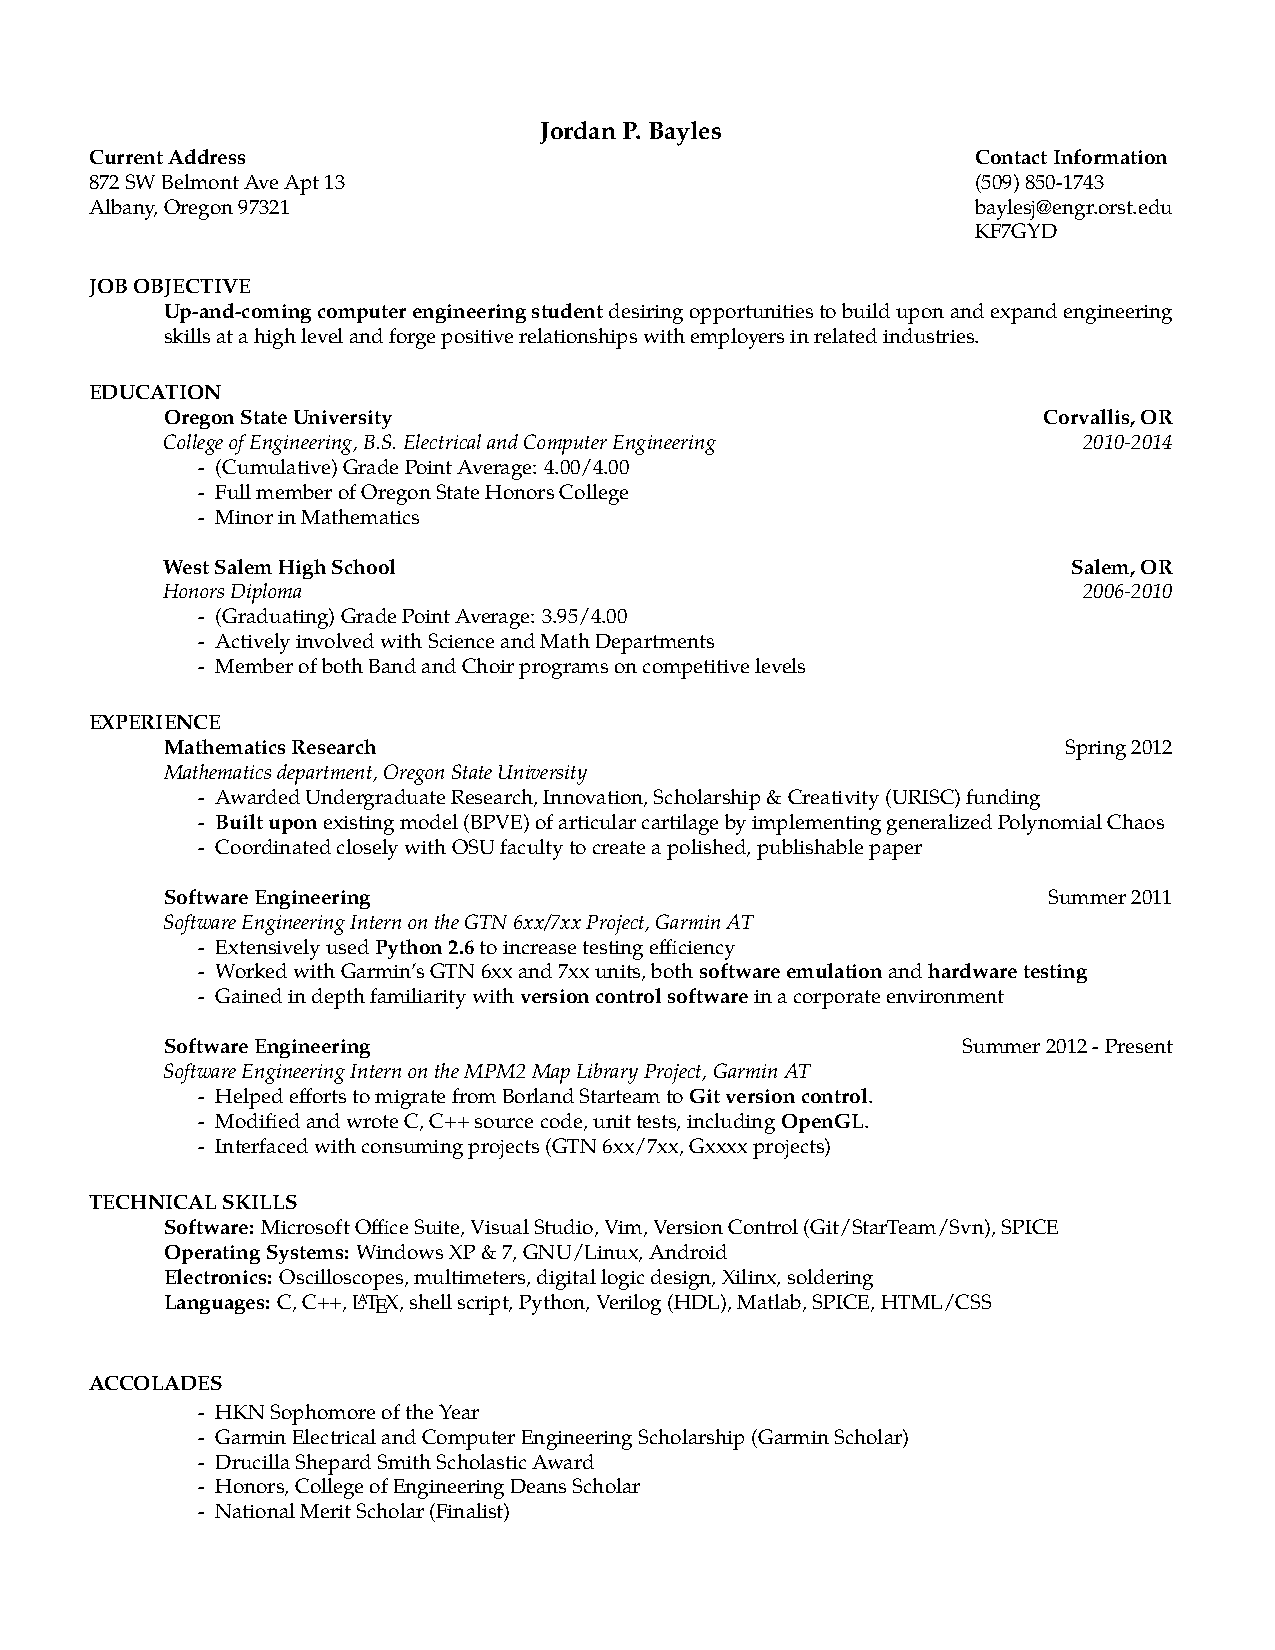
\includepdf[pages={1}]{resume.pdf}

\end{document}
